\documentclass[10pt,twocolumn,letterpaper]{article}

\usepackage{cvpr}
\usepackage{times}
\usepackage{epsfig}
\usepackage{graphicx}
\usepackage{amsmath}
\usepackage{amssymb}
\usepackage{float}
\usepackage{caption}


% Include other packages here, before hyperref.

% If you comment hyperref and then uncomment it, you should delete
% egpaper.aux before re-running latex.  (Or just hit 'q' on the first latex
% run, let it finish, and you should be clear).
\usepackage[breaklinks=true,bookmarks=false]{hyperref}

\cvprfinalcopy 

\def\httilde{\mbox{\tt\raisebox{-.5ex}{\symbol{126}}}}
\graphicspath{ {pictures/} }
\setcounter{page}{1}
\begin{document}

%%%%%%%%% TITLE
\title{Spotting Distracted Drivers Using Classic CV Methods}

%%%%%%%%% Author Names
\author{Guillermo Reyes\\
{\tt\small enggreys@gmail.com}
\and
Daniel Schaefer\\
{\tt\small secondauthor@i2.org}
\and
Marc Tonsen\\
{\tt\small secondauthor@i2.org}
\and
Dominik Weber\\
{\tt\small secondauthor@i2.org}
}

\maketitle

%%%%%%%%% ABSTRACT
\begin{abstract}
   The ABSTRACT is to be in fully-justified italicized text, at the top
   of the left-hand column, below the author 
   information. Use the word ``Abstract'' as the title, in 12-point
   Times, boldface type, centered relative to the column, initially
   capitalized. The abstract is to be in 10-point, single-spaced type.
   Leave two blank lines after the Abstract, then begin the main text.
\end{abstract}

%%%%%%%%% BODY TEXT

\section{Introduction}
According to the U.S. Department of Transoprtation and National Highway Traffic Safety Administration, about 18\% of all injury crashes and 10\% of fatal crashes are reported to involve distracted drivers at the moment of the accident ~\cite{knuthwebsite}. This, unfortunately, translates to over 3000 people killed and 400,000 injured per year, in the United States alone due to motor vehicle crashes.

This clearly speaks for measures to be taken. Spotting distracted drivers in time could help to take appropriate actions and thus prevent accidents and save thousands of lives each year. In order to detect distracted drivers, different approaches have been taken. However, many of them and intrusive and expensive. However by using simple cameras combined with computer vision algorithms, one can get a solution that is both cheap and non-intrusive.

For this task we have entered the Kaggle Competition: State Farm Distracted Driver Detection ~\cite{Kaggle}. The challenge consists of classifying images of drivers engaging in the behaviors described below.

\begin{enumerate}
	\item Safe driving
	\item Texting with right hand
	\item Talking on the phone with right hand
	\item Texting with left hand
	\item Talking on the phone with left hand
	\item Operating the radio
	\item Drinking
	\item Reaching behind
	\item Hair and makeup
	\item Talking to passenger
\end{enumerate}

The competition provides the dataset with over 2000 training images per class, 26 different drivers with diverse ethnic backgrounds, in 4 distinct cars and camera angles and distinctive lighting conditions as well as some noise in the data.

In this paper we propose different approaches to solve this task using some classic computer vision methods to find out how well they stack up against state of the art methods such Deep Neural Networks, which can already achieve up to 99\% accuracy .


\section{Related Work}



\section{Proposed Method}

\subsection{HOG Landmarks}
For last approach used in this paper, we look for specific things in the images that help us make a decision. We call these specific things landmarks. A landmark can be anything in the images(pose, objects, etc.) that can be used to distinguish a class from the others. These landmarks are chosen arbitrarily in this paper and we shall later evaluate how well they perform. Below we outline what of these landmarks are, note that there is at least one distinctive landmark per class.

\begin{enumerate}
	\item Head facing front, towards the road.
	\item Head facing sideways towards the copilot
	\item Head facing backwards towards the back passengers.
	\item Empty gap in front of the head rest
	\item Right hand holding phone while texting
	\item Right hand holding phone while talking\
	\item Left hand holding phone while texting
	\item Left hand holding phone while talking
	\item Hand holding bottle/cup
	\item Hand near head
	\item Hand reaching behind
	\item Hand reaching for radio	
\end{enumerate}




First off, we have taken approximately 50 images per class have manually labeled the bounding boxes around the selected landmarks. We then proceeded to train a detector based on HOG features for each of the landmarks with  help of Dlib \cite{dlib09}. 



%\begin{minipage}[t]{.5\textwidth}
%	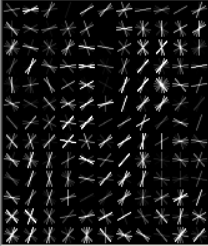
\includegraphics[width=\textwidth]{mult_HOG/HOG_phone}
%	\captionsetup{justification=raggedright, singlelinecheck=false}
%	\captionof{figure}{H Feistel Function}
%\end{minipage}%
%\begin{minipage}[t]{.5\textwidth}
%	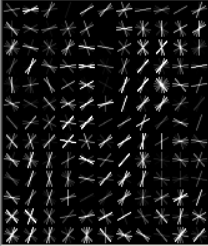
\includegraphics[width=\textwidth]{mult_HOG/HOG_phone}
%	\captionsetup{justification=raggedright, singlelinecheck=false}
%	\captionof{figure}{HOG of the right hand holding phone while texting landmark}
%\end{minipage}


%\begin{figure*}[h]
%	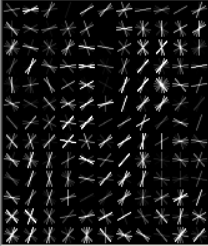
\includegraphics[width=0.85\columnwidth]{mult_HOG/HOG_phone}
%	\captionsetup{justification=raggedright,
%		singlelinecheck=false
%	}
%	\caption{HOG of the right hand holding phone while texting landmark}
%\end{figure*}



\section{Experimental Results}

\subsection{HOG Landmarks}




\section{Conclusion}

\section{Future Work}



%%%%%%%%% REFERENCES

{\small
\bibliographystyle{ieee}
\bibliography{egbib}
}

\end{document}
